%!TEX root = ../thesis.tex

% *****************************************************************************
% ********************************** CHAPTER 2 ********************************
% *****************************************************************************

\chapter{Board Characteristics}

This chapter goes into an in-depth exploration of the AM64x board, showing the
major features exploited during the realization of the project.
The chapter begins with the reasons behind the selection of the board.
Next, the chapter explores through a comprehensive analysis of the
distinctive processor characteristics of the AM64x board: the Arm Cortex-A53,
Cortex-R5F, Cortex M4 and PRU cores. The analysis of the processors shows their
individual attributes and how they can work together to solve more complex
tasks.
Furthermore, the discussion will explore the mechanisms for interprocessor
communication, which is a core concept for the coordination among the
heterogeneous cores.

\section{Board Selection}

The first task done during the internship was the selection of the board to use
during the project.
Different boards were analyzed during this process, each with its own set of
characteristics.

\begin{figure}
    \centering
    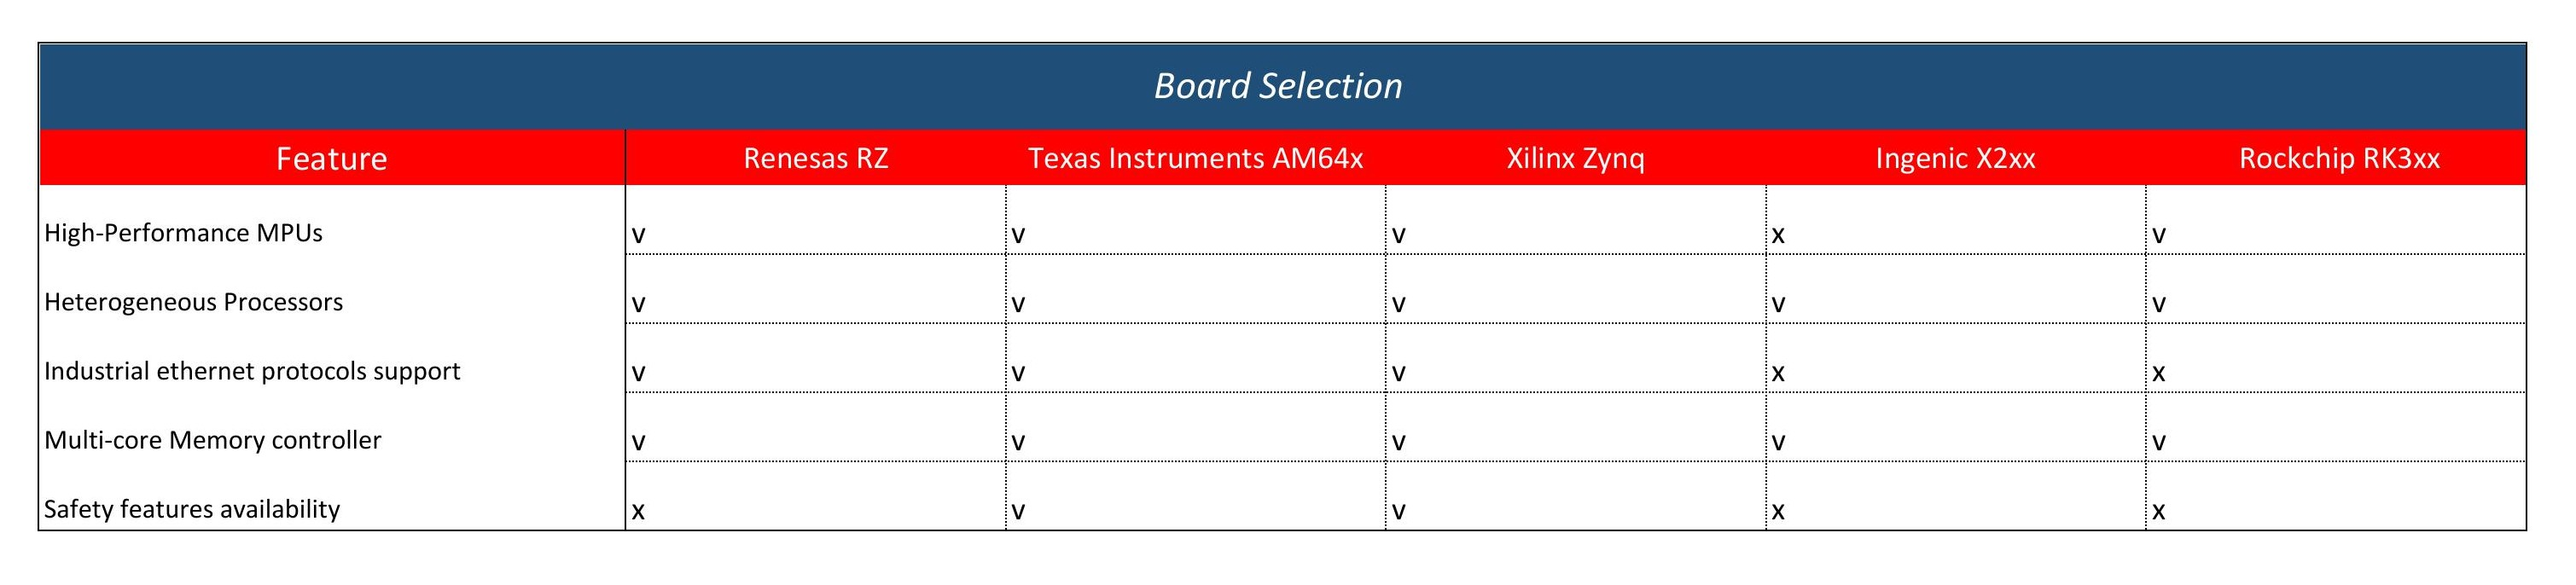
\includegraphics[height=5cm, width=1.0\textwidth]{Figures/board_selection.jpg}
    \caption{Board analyzed}
\end{figure}

The AM64x was the only board which met all the criteria, making it the perfect
candidate for this project.

The first important element was the availability of different heterogeneous
cores. The AM64x board has heterogenous multi-core architecure, offering a
spectrum of processing cores like: Arm Cortex-A53, Cortex-R5F, Cortex-M4F and
PRU cores. This diversity in processing capabilities enables the implementation
of complex algorithms and tasks across different computational requirements.

Another important factor is the board's native support for Ethernet
communication, including Gigabit Ethernet ports and protocols to guarantee 
seamless data exchange between the embedded system and external devices,
facilitating efficient communication with regular PCs.

Additionaly, the board's robust hardware features, such as: large connectivity
options, extensive peripheral support, and integrated security features,
complement the application's demands in orchestrating reliable and secure
communication in heterogeneous environments.

\section{Introduction to AM64x}

AM64x is an extension of the Sitara industrial-grade family of heterogeneous
Arm processors. \cite{AM64_datasheet}
AM64x is designed for applications in industrial automation, industrial
communication, and other embedded systems application which require a unique
combination of real-time processing and communications with application
processing. 

AM64x combines two instances of Sitara's gigabit TSN-enabled PRU-ICSSG,
two Arm Cortex-A53 cores, four Cortex-R5F MCUs, and a Cortex-M4F MCU
domain.

\begin{figure}[htb]
    \centering
    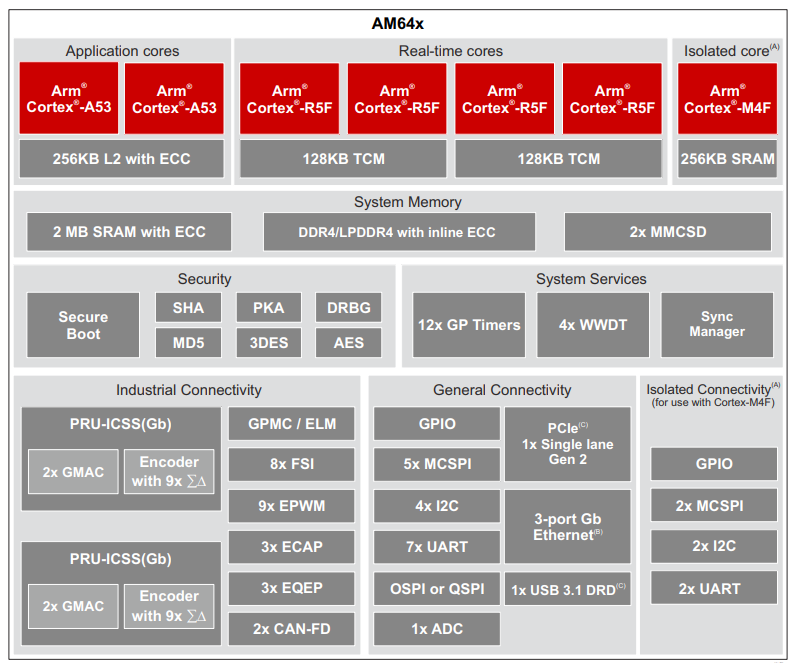
\includegraphics[width=1.0\textwidth]{am64_architecture.png}
    \caption{AM64x architecture}
\end{figure}

The Arm Cortex-A53 Cores are specifically optimized for higher-level
processing tasks.
They offer good performance for general-purpose computing and serving as a
popular choice for running operating systems, such as embedded Linux.
Their computational power enables the fusion of the Linux environment with the
real-time capabilities offered by the other cores within the AM64x.
The AM64x offers configurable memory partitioning, facilitating the division
of memory allocation between the Linux cores and the real-time cores.
Particularly, the Cortex-A53s can exclusively utilize DDR memory, while 
the internal SRAM can be flexibly allocated in various sizes to accomodate
the needs of the Cortex-R5fs, either collectively or individually.

Within an embedded system, the most important objective is to provide real-time
computation, and this is done through the high performance R5Fs, in the AM64x.
Arm Cortex-R5F cores offers a robust set of real-time processing capabilities
wihch are fundamental for deterministic and time-critical tasks.
These cores are specifically designed to handle real-time operations, ensuring
precise timing, reliability, and responsiveness in applications within embedded
systems and industrial environments.
The functionalities best suited for the R5Fs are those requiring deterministic
behavior, such as control systems, motor control, and real-time monitoring.
Their architecture is also optimized for safety operations, guaranteeing 
reliability and predictability in execution.
As highlighted in the introduction, this is one of the most important aspect
in the industrial automation applications.
Moreover, the inclusion of quad-core Cortex-R5Fs in the AM64x provides the
possibility of parallel processing, allowing for efficient handling of multiple
real-time tasks simultaneously. The multi-core setup enhances the system's
ability to manage complex control algorithms or handle several concurrent
real-time processes without compromising performance or reliability.

The integrated Cortex-M4F core, coupled with dedicated peripherals within the
AM64x series, enables the implementation of functional safety features,
which is a crucial characteristic in many industries.
The possibility of isolating these safety-critical elements from the rest
of the SoC guarantees enhanced security and integrity.

The M4F core is developed to address digital signal control markets that demand
an efficient, easy-to-use blend of control and signal processing capabilities.
\cite{ARM_M4}
The combination of high-efficiency signal processing functionality with the
low-power, low cost and ease-of-use benefits of the Cortex-M family of
processors satisfies markets.

Finally, in the architecture of the AM64x can be found an additional
co-processor called PRU-ICCSG (Programmable Real-Time Unit for Industrial
Communication SubSystem Gigabit). This subsystem is used for industrial
communication, being able to perform real-time industrial communication.
PRU cores are primarily sed for industrial communication, but they can also
be used for other applications such as motor control and custom interfaces.
The PRU-ICSSG frees up the main ARM cores in the device for other functions,
such as control and data processing.

\subsection{A53 Subsystem}

The SoC implements one cluster of dual-core Arm Cortex-A53 MPCore, which is
a multi-core variant of the A53 core, where each core can execute code 
independently from the other.
It is based on the symmetric multiprocessor (SMP) architecture, where all
cores have equal access to system resources like memory and peripherals.


\begin{figure}[htb]
    \centering
    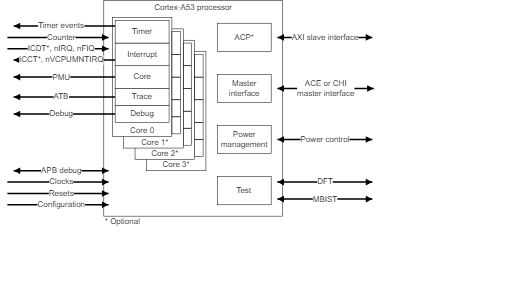
\includegraphics[width=1.0\textwidth]{A53_MPCore_architecture.png}
    \caption{Cortex-A53 MPCore architecture with 4 cores}
\end{figure}

The Cortex-A53 processor is a high efficiency processor that implements the
Armv8-A architecture. While maintaining the A53's energy efficiency, the
Cortex-A53 MPCore enhances overall system performances through parallel
processing.

The A53 CPU has the ability to execute 64-bit applications with the AArch64
execution state. It also has the possibility to execute 32-bit applications
with the AArch32 state for retrocompatibility with the existing ArmV7-A
applications.

\begin{figure}[htb]
    \centering
    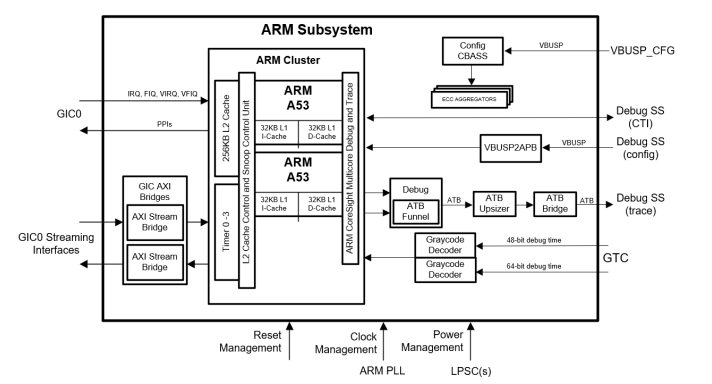
\includegraphics[width=1.0\textwidth]{A53_diagram.png}
    \caption{A53SS Block Diagram}
    \label{fig:A53_diagram}
\end{figure}

Each core within the subsystem is equipped with 32KB L1 instruction and 32KB
L1 data caches, complemented by a shared 256KB L2 cache, as illustrated in
Figure \ref{fig:A53_diagram}. These cache configurations significantly
contribute to optimizing data access and enhancing overall processing
efficiencty.

Given the processing power of the Cortex-A53 core, it is usually used to run
embedded Linux and combine the features offered by Linux with the real-time
operations offered by the other cores.
In this idea, the A53 can be used for general purpose computing and interact
with the other cores to execute certain services which require to satisfy
real-time contraints.

\subsection{R5F Subsystem}

The board selected for the project has two R5F subsystems, a dual-core
implementation of the R5F processor, which is a version of the R5 processor
with the floating point unit extension.

\begin{figure}[ht]
    \centering
    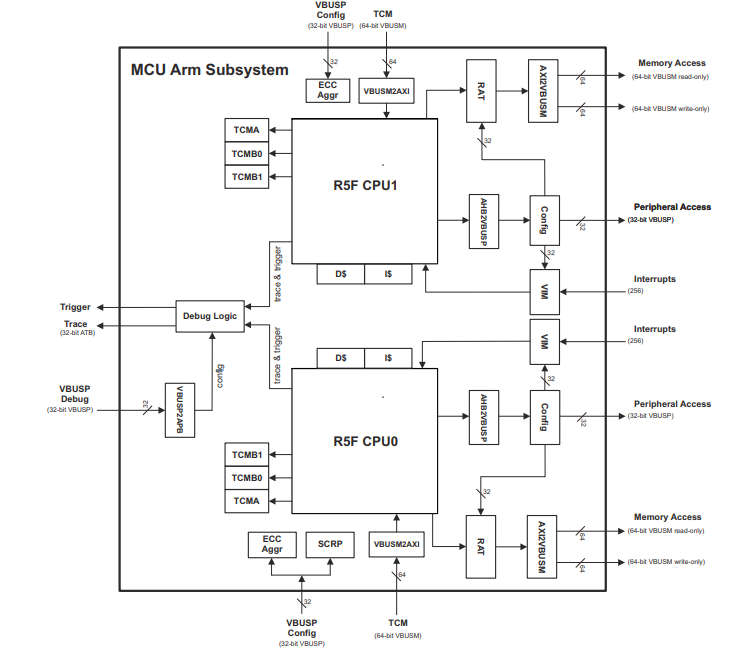
\includegraphics[width=1.0\textwidth]{R5FSS_diagram.png}
    \caption{R5FSS Block Diagram}
\end{figure}

The architecture of the R5F core is the Armv7-R, which is specifically designed
for real-time applications.
The most important features are: deterministic behavior, safety and
reliability.

It features an Harvard memory architecture, which separates the cache for
instructions and the cache for data.
Each core has a total of 32KB of L1 cache: 16KB for instruction and 16KB for
data.

To enable fast memory access the R5F has two tightly-coupled memories (TCMs),
which are low latency, tightly integrated memories that can be used for
instructions or data. The total TCM available for each core is of 32KB.
It has similar performance to accessing instructions or data in cache.
\cite{Technical_reference_AM64}

One of the most important features of the TCMs is the possibility to be
accessed from external sources. This makes possbile to preload data in the
memory, such as instructions before they are needed from the core.
It is also possible to process data and save it on the TCMs, and external
sources can directly access the data, without communicating with the core.

The TCM can be used to hold time-critical routines, such as interrupt
handling routines or real-time tasks where the indeterminacy of a cache is
undesirable. In addition, you can use it to hold ordinary variables, data types
whose locality properties are not well suited to caching, and critical data
structures such as interrupt stacks. \cite{TCM_documentation}

The subsystem can operate in one of two modes: split or single-core mode, which
has to be decided during bootstrap.
In split mode, each core of the subsystem is considered as a standalone
processor, working completely independent from the other, and each of them has
dedicated RAMs and interfaces.
In single-core mode, only one of the cores is operating, but it has available
the TCM of the second core, which could be offered advantages in performance if
the processing power of two cores is not needed, but a lot of data has to be
processed. 

\subsection{M4F Subsystem}

The last core of the system is an Arm Cortex-M4F running safety processing.
Similar to the R5F, also the M4F has the extension for floating point unit.

\begin{figure}[ht]
    \centering
    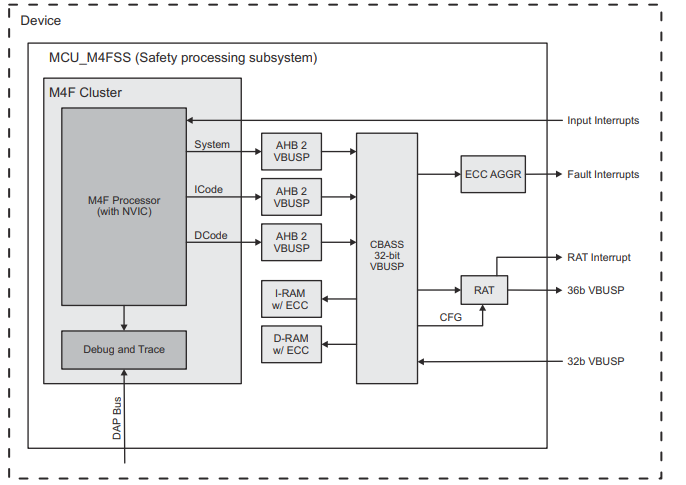
\includegraphics[width=1.0\textwidth]{M4FSS_diagram.png}
    \caption{M4FSS Block Diagram}
\end{figure}

The Cortex-M4F processor is a low-power processor that features low gate count,
low interrupt latency, and low-cost debug. This processor is intended for
deeply embedded applications that require fast interrupt response features.
\cite{M4F_technical_reference}
The processor delivers exceptional power efficiency through an efficient
instruction set and extensively optimized design. The M4 processor implements
a version of the Thumb instruction set based on Thumb-2 technology, ensuring
high code density and reduced program memory requirements.

The M4FSS has a total of 256Kb of SRAM divided into two banks: 192KB of I-RAM,
and 64KB of D-RAM. The I-RAM meory is intended mainly for M4F's instruction
code, and D-RAM for M4F's data. The M4F allows concurrent fetch for instruction
code and data via dedicated buses.
The M4FSS supports unified memory for both banks, which means that instruction
code and data can be placed in any bank, although, it is recommended that
the data saved is the intended one for efficiency purposes.

The RAM also has Error-correcting code (ECC), which is used to detect and
correct data corruption which occurs in memory.
To enhance safety, the core also has a Memory Protection Unit (MPU), giving
the possibility to privileged software to define memory regions and assign
memory access permission and attributes to each of them.

The M4FSS incorporates a dedicated local reset input. This makes possible to
preload code in the M4F RAM and then release the reset, in this way the
processor will have the instructions it needs when it starts.

During the boot sequence, another processor will start the M4F, from that point
onward the M4F will be isolated form other cores, running safety processing.
This isolation from other cores on the board is important to maintain a highly
secure and predictable compuational environment, essential for safety-critical
applications.

\subsection{PRU-ICSSG}

Industrial communication within Sitara proessors and microcontrollers is
efficiently managed by the Programmable Real-Time Unit Industral Communication
Subsystem (PRU-ICSS). The PRU-ICSS is a co-processor subsystem that houses the
PRU cores and Ethernet media access controllers (EMACs), responsible for
executing low-level industrial Ethernet and fieldbus protocols via firmware.
Higher-level protocol stack components are implemented in software running on
the Arm cores.

PRU cores are mainly dedicated to industrial communication but can be harnessed
for other custom applications, freeing the main Arm cores for more general
control and data processing.

\begin{figure}[ht]
    \centering
    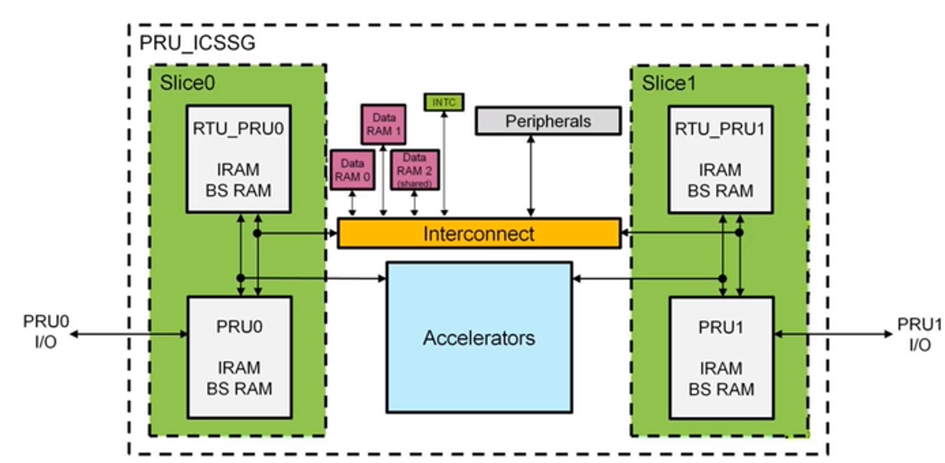
\includegraphics[width=1.0\textwidth]{PRUICSSG_architecture.png}
    \caption{PRUICSSG Architecture}
\end{figure}


PRU-ICSSG represent the next generation of PRU-ICSS, building on the
capabilities introduced in the predecessor (PRU-ICCS).
At its core, each PRU-ICSSG has 4 32-bit RISC cores:

\begin{enumerate}
    \item 2 PRU cores
    \item 2 Auxiliary Programmable Real-Time Units known as RTU-PRUs
\end{enumerate}


A notable enhancement in the PRU-ICSSG, compared to its predecessor, is the
inclusion of internal accelerators. These accelerators play a crucial role in
data processing and movement, contributing to the achievement of both real-time
and Gigabit-level speeds.

\subsubsection{PRU-ICSSG Cores}

PRUs, or Programmable Real-Time Units, are specialized processing units
embedded in the Sitara family of microcontrollers. PRUs are designed for
real-time applications that require low-latency and deterministic performance.
They offer a dual-core architecture, with high programmability, enabling custom
firmware to be executed in real time. PRUs are especially suitable for tasks
such as industrial control, motor control, communication interfaces, and custom
I/O control. They provide low-latency, direct access to processor pins, making
them efficient for interfacing with external devices. PRUs can be used
alongside the main ARM CPU, sharing resources as needed.

Within the subsystem there are two type of cores: PRUs and RTUs. The key
distinction between them lies in their I/O access. PRUs are versatile,
capable of I/O control and data processing, while RTUs are exclusively
designated for data processing. Both, however, share access to PRU\_ICSSG and
SoC resources.

The PRU-ICSSG is divided in two symmetrical slices. Each of them containing
one PRU core and one RTU\_PRU core.
The content within each slice is only accessible to the PRU and RTU cores
within that slice, whereas content outside the slices can be accessed by any
core.
Each core has its dedicated instructions and broadside RAM, along with a RAM
dedicated to each slice, shared by the cores belonging to that slice.

Each core can operate independently or in coordination with ARM cores or other
PRU/RTU cores.

PRU cores are designed as non-pipelined, single-cycle execution engines. This
means that all instructoins, except for memory reads and writes, are completed
within a signle cycle. As there is no pipelining, PRU cores offer full
determinism, ensuring that instructions are not rearranged during execution.

\section{Memory Map Layout}

The memory map of an embedded device provides a layout of the memory space,
indicating how different types of memory are organized and used within the
device.

The two most important types in the AM64x are: MSRAM and DDR memory layout.

\subsubsection{MSRAM}

MSRAM, or SRAM (Static Random-Access Memory), stands out of its high speed,
low power consumption when idle, reliability, and lack of a need for data
refreshing. However, it's relatively expensive and offers lower storage
densite compared to DDR SDRAM.

The AM64x SoC offers a total of 2MB of MSRAM, divided into eight individual
banks, each with a size of 256KB.

Each of the four R5s cores has access to dedicated 256 KB private bank for
exclusive use, providing isolation and dedicated memory space for each core.

In addition to core-specific banks, there are shared banks accessible by all
cores, facilitating inter-core communication, shared data storage, and support
for applications requiring more memory than their private banks can offer.
Shared banks play an important role in enabling communication and data sharing
between different cores within the SoC, providing collaborative processing
capabilities.

This memory layout offers flexibility for applications. When using only one
core, applications can utilize the private banks reserved for other cores as
needed.

\begin{figure}[ht]
    \centering
    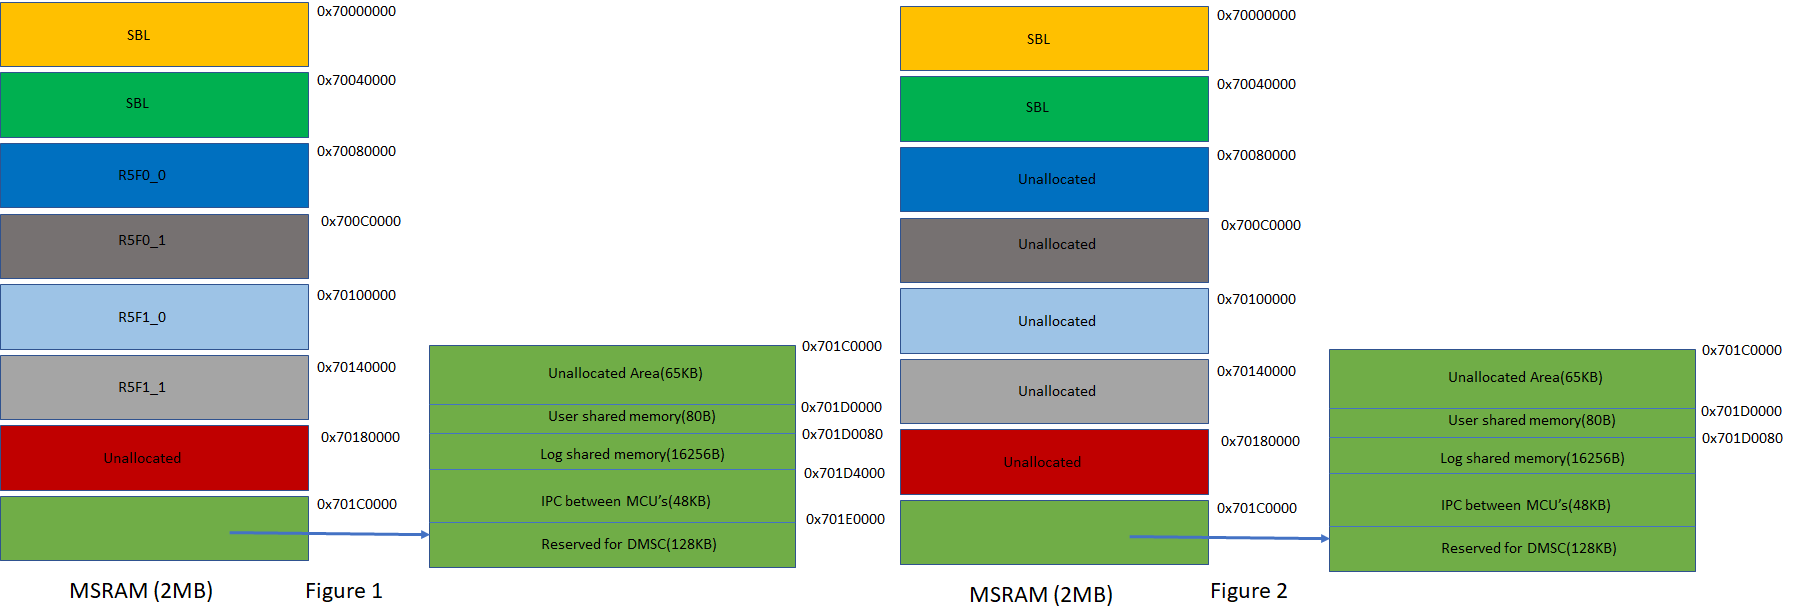
\includegraphics[width=1.0\textwidth]{MSRAM_layout.png}
    \caption{MSRAM layout}
\end{figure}

The first 512 KB of MSRAM is set aside for a specific purpose, it's reserved
for the System Bootloader (SBL). The SBL is responsible for initializing the
system, and it contains essential elements such as the System Controller
Firmware (SYSFW) and SYSFW Board Configuration data.

The reason this memory is reserved is to create a dedicated space for the
combined bootloader image. This image ensures that SYSFW is properly loaded
into the DMSC Cortex M3 processor. Any attempt to modify or use tihs reserved
memory for other purposes in the linker file should be avoided. If the
reserved area is accidentally overlapped with an application's memory space,
it can lead to problems during the boot process.
Specifically, during the boot process, the SBL loads the core image, and if the
reserved memory is not respected, there's a risk of overwriting the SBL itself.
This could result in a malfunctioning or unstable system. To prevent such
issues, the SBL has built-in checks that will flag an error if it detects any
section of an application falling within the reserved memory region. These
checks are in place to ensure the system's integrity and reliable boot-up.

\subsubsection{DDR}

DDR is known for its high data throughput, cost-effectiveness, synchrnous
operation with the system clock, and data transfer on both edges of the clock
signal. This double data rate transfer significantly increases bandwidth and
is ideal for memory-intensive applications. DDR SDRAM also provides greater
memory density compared to MSRAM.

The layout of the DDR differs, depending on which Operating System is running
on the cores.

If embedded Linux is running on the A53 core, the DDR is divided into sections,
one for every core, which has to be used in the RTOS application.

\begin{figure}[ht]
    \centering
    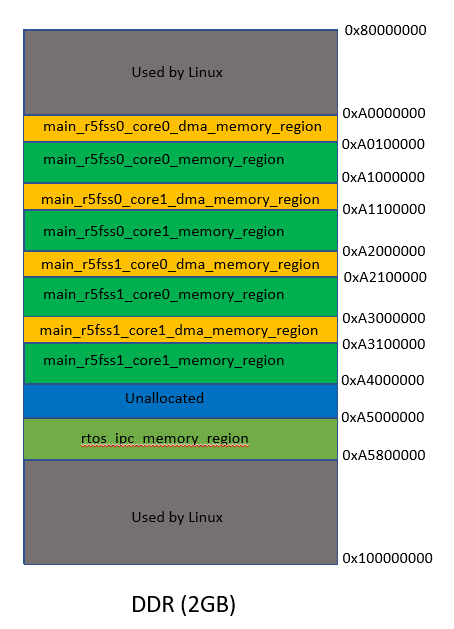
\includegraphics[width=0.5\textwidth]{DDR_linux.png}
    \caption{DDR layout with linux running on A53 core}
\end{figure}

If an RTOS or a bare-metal application is running on the A53 core, the
application needs to be loaded into DDR for booting.
The DDR is not allocated in this case, and it can be used by the all the cores,
specifying it in the linker file.

\begin{figure}[ht]
    \centering
    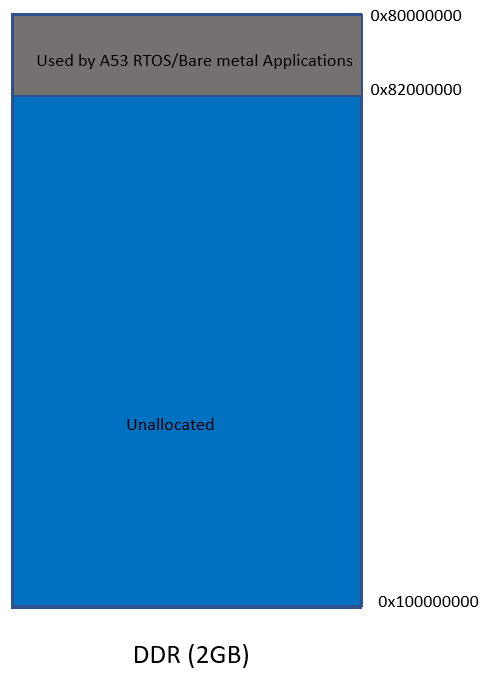
\includegraphics[width=0.5\textwidth]{DDR_without_linux.png}
    \caption{DDR layout with RTOS or baremetal application on A53 core}
\end{figure}

\section{Networking}

Advances in the embedded systems have led to new functionalities to be
required. The ability to communicate over the internet with other devices.

Networking is a broad term used to cover Ethernet (IEEE 802.3), EtherCAT
Profinet and other ethernet-like communication protocols used in industrial,
automative and other general use cases.

Networking is supported using the following hardware peripherals:

\begin{itemize}
    \item   Common Port Switch (CPSW): CPSW subsystem provides IEEE 802.3
            standard Ethernet gigabit speed packet communication for the
            device and can also be configured as an Ethernet switch.
            CPSW supports RGMII and RMII interfaces.
    
    \item   PRU-ICSSG: PRU-ICSSG is firmware programmable and can take on
            various personalities like Industrial Communication Protocol Switch
            (for protocols like EtherCAT, Profine, EtherNet/IP), Ethernet
            Switch, Ethernet MAC, Industrial Drives, etc. PRU-ICSSG supports
            RGMII and MII modes.
\end{itemize}

\begin{figure}[ht]
    \centering
    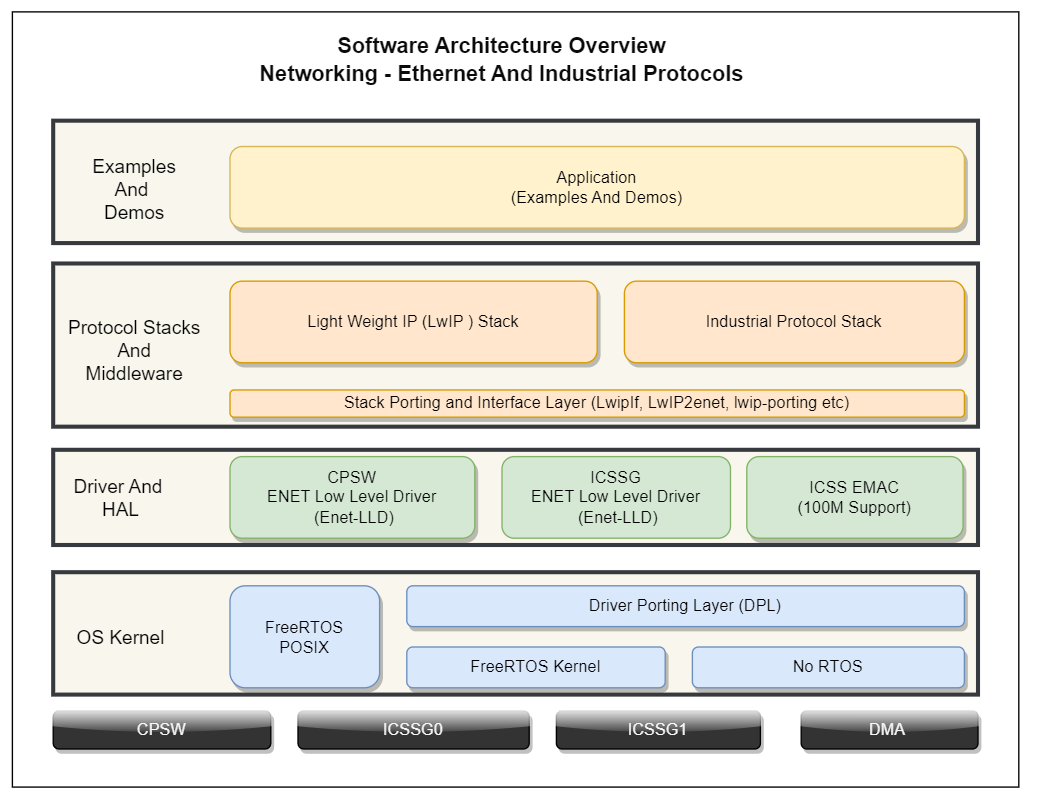
\includegraphics[width=1.0\textwidth]{networking_software_architecture.png}
    \caption{Networking Software Stack}
\end{figure}

\section{Inter Processor Communication}

Inter-Processor Communication (IPC) is a fundamental aspect of multi-core
systems like the AM64x SoC. In such systems, multiple CPUs or processor cores
works together to achieve specific tasks or run various applications.
These cores may need to communicate and share daa with each other to realize a
larger system-level application or to coordinate their activities.
IPC mechanisms facilitate this communication.

\begin{figure}[ht]
    \centering
    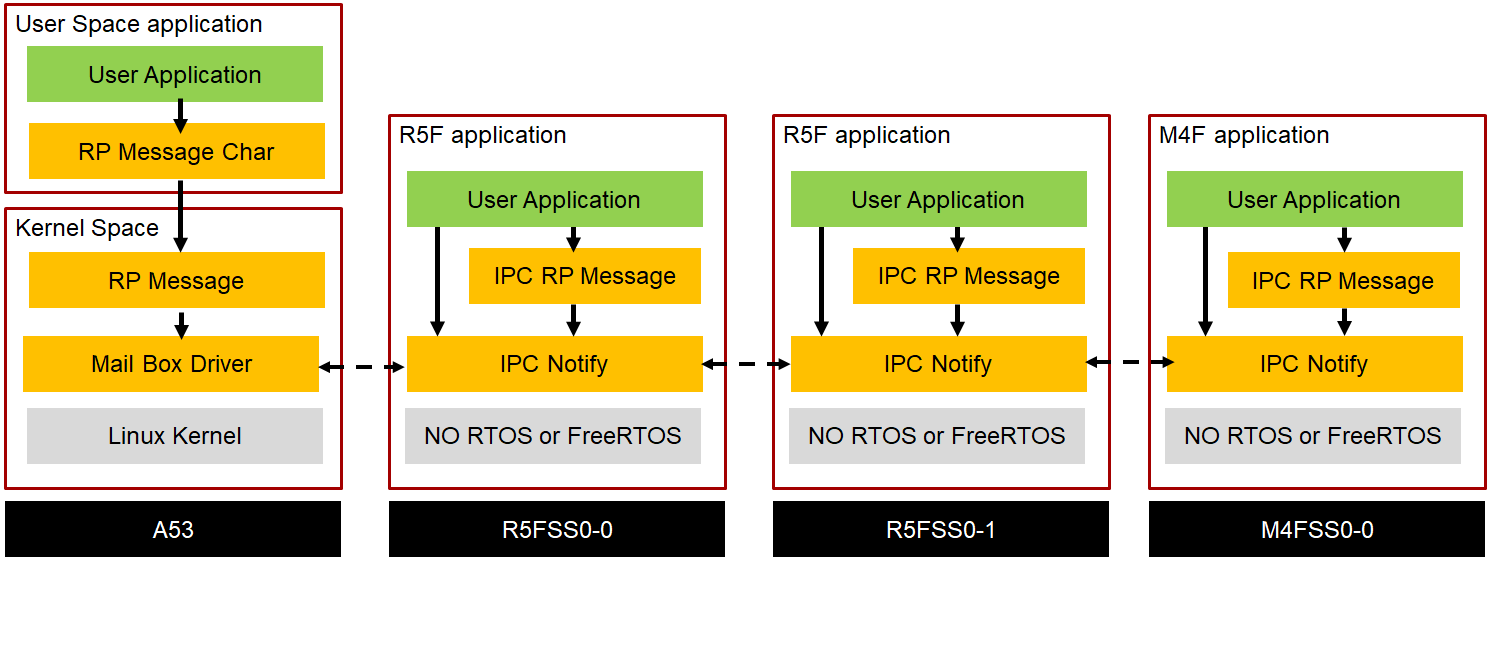
\includegraphics[width=1.0\textwidth]{IPC.png}
    \caption{IPC mechanisms}
\end{figure}

There are two IPC mechanisms to realize communication between real-time cores:

\begin{enumerate}
    \item   IPC Notify
    \item   RPMessage
\end{enumerate}

Developers can leverage IPC Notify alongside RPMessage, to fine-tune their
applications based on their specific needs and requirements.

\subsection{IPC Notify}

IPC Notify defines APIs for enabling low-latency inter-processor communication
between different CPU cores. These APIs prioritize speed and efficiency and are
therefore constrained in terms of features.

To achieve low latency, the underlying implementation employs hardware
mechanisms to interrupt the receiving CPU cores. Additionaly, it utilizes
hardware FIFOs when available, and in cases where hardware FIFOs are not
present, it resorts to using software FIFOs based on fast internal RAM to
transport message values.

In the case of AM64x, IPC notify utilizes hardware mailbox-based hardware FIFOs
to transport messages and interrpt the receiving CPU core.
This approach ensure that messages are exchangesd with minimal delay and high
efficiency, making it suitable for scenarios where speed is a primary
consideration.

The first limitation to have all the advantages offered by IPC notify is the
size of the message: IPC Notify combines the message content and client ID into
a single 32-bit value, limiting the content of the message to less than a byte.

\subsection{RPMessage}

RPMessage, or Remote Processor Message, is a communication method that enables
CPUs to exchange messages in the form of packet buffers. These messages are
directed to specific logical endpoints on another CPU, facilitating efficient
inter-processor communication.

RPMessage exploits shared memory between cores to exchange the messages.
The sender places a packet in a buffer inside the shared memory. After that,
it has to notify the receiving core that there is a new message to process.
This notification is done using a hardware interrupt mechanism, similar to
IPC Notify.

In contrary with IPC Notify, RPMessage allows for variable packet sizes.
When both ends are using real-time operating systems, the minimum packet size
is 4 bytes, but it can be configured by the developer to use bigger sizes,
although 512 bytes should be taken as upper limit.
If Linux is involved in the communication the size of the packet is fixed to
512 bytes, configured in the Linux kernel.

Every core can establish multiple logical endpoints, where the message can be
delivered to, allowing for multiple communication channels between CPUs.

\subsection{Linux IPC}

The RPMsg char driver serves as an interace for user-space processes to
access RPMsg endpoints. These endpoints are used for communication between
different applications and can be uniquely accessed by requesting specific
interactions with the remote service. What is important to note is that the
RPMsg char driver supports the creation of multiple endpoints for each RPMsg
char devicce that has been initialized. This means that a single RPMsg char
device can be used for different instances or applications.

When these endpoints are created, they appear as individual character devices
within the /dev directory. Underlying this setup, the RPMsg bus operates on top
of the VirtIO bus. Each time a VirtIO name service announcement message is
sent, a new RPMsg device is generated, and it is intended to be bound to an
RPMsg driver. These RPMsg devices are dynamically generated, initiated by an
announcement message from the remote processor. This message contains
information about the service's name, source, and destination addresses.

The handling of this announcement message is the responsibility of the
RPMsg bus, which dynamically creates and registers an RPMsg device that
represents the remote service. Once a relevant RPMsg driver is registered, it
is immediately probed by the bus, and this allows both sides to begin
exchanging messages.

\begin{figure}[ht]
    \centering
    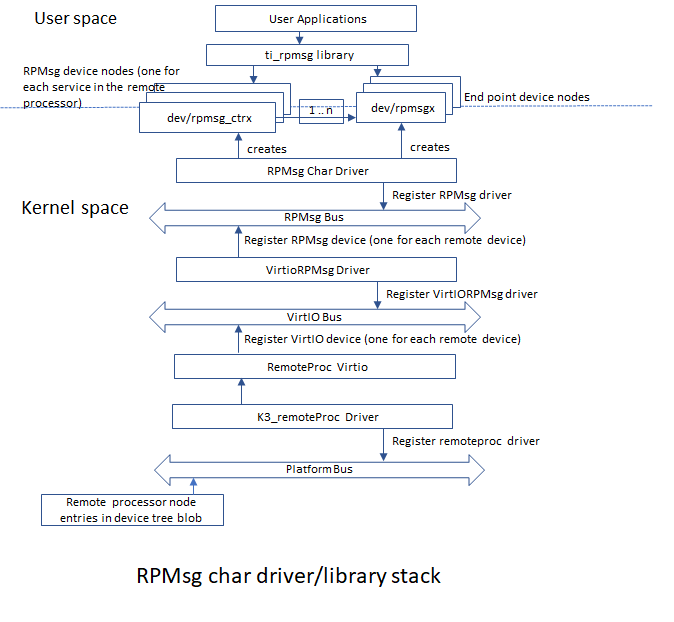
\includegraphics[width=0.8\textwidth]{RPMsg_stack.png}
    \caption{RPMsg library stack}
\end{figure}

\subsection{PRU IPC}

Given that PRUs can offload tasks from the primary cores, establishing 
communication between the PRU cores and the ARM cores becomes essential.

PRU IPC module provides APIs for communicating with the PRU cores with low
latency. The communication is done in the form of blocks of data transfer in
one exchange. Options are available for configuring multiple buffers and blocks
per buffer.

\begin{figure}[ht]
    \centering
    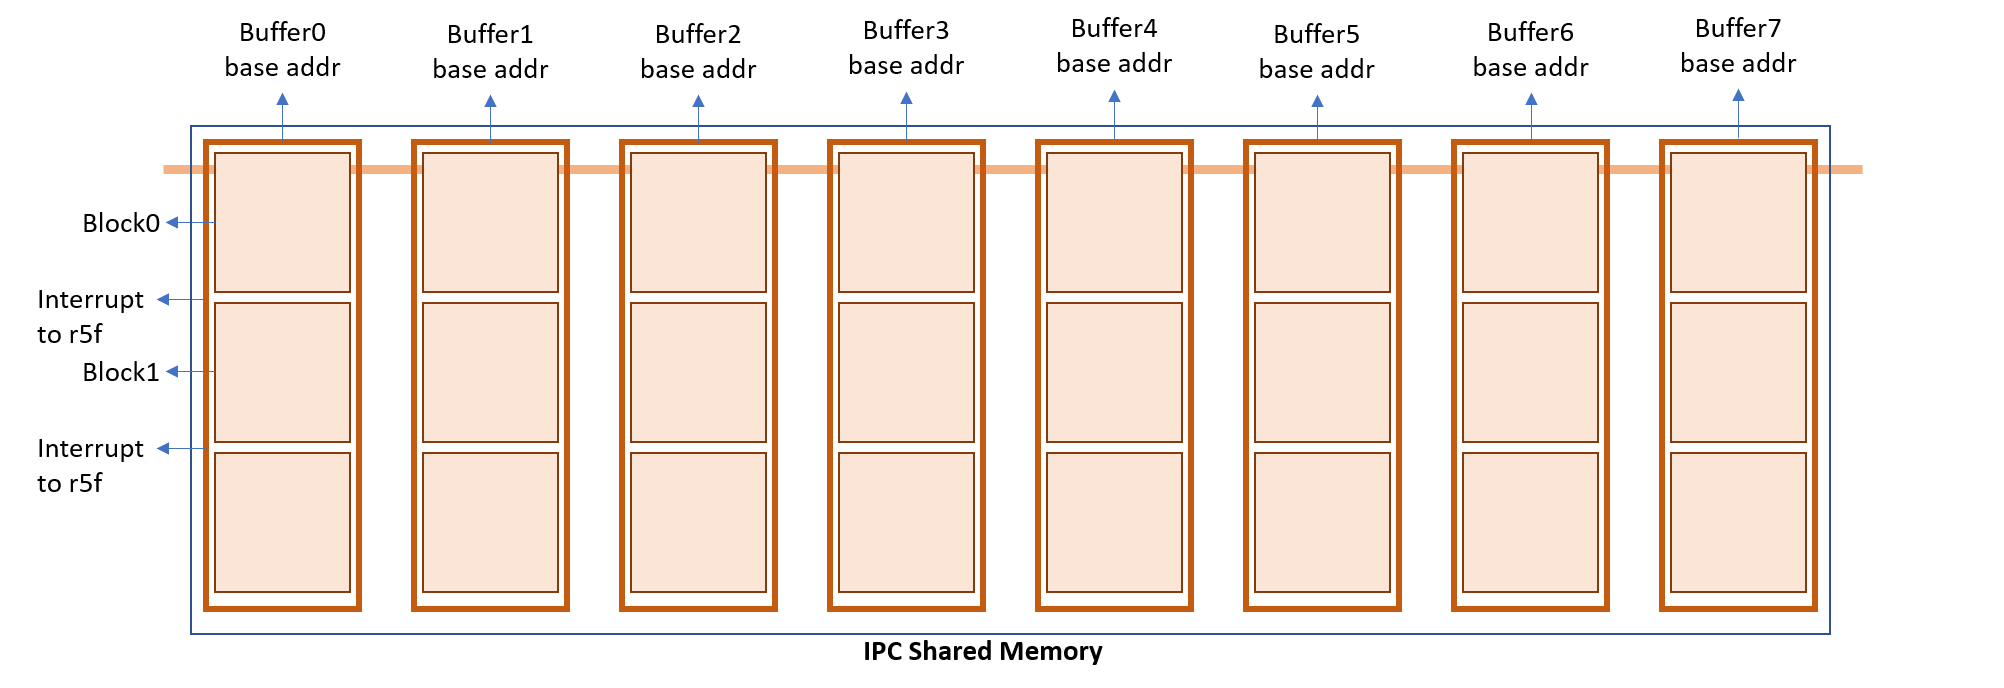
\includegraphics[width=0.8\textwidth]{IPC_PRU.png}
    \caption{PRU IPC}
\end{figure}

PRU write to the shared memory and creates an interrupt even once a certain
number of samples, which are equal to the block size, have been written into
IPC Shared Memory.
The PRU writes one block of data for all the buffers at a time, and then moves
on to the buffer after that.

After writing the block of data, the PRU sends an interrupt to the destination
of the message, which can read it from the shared memory.

\subsubsection{Communication between Linux and PRUs}

There are two vrings provided per PRU core, one vring is used of rmessages
passed to the Linux core and other one is used for receiving messages.
System level mailboxes are used to notify cores (ARM or PRU) when new messages
are waiting in the shared buffers.

On the ARM Linux side, RPMsg messages are received in kernel space.
An interface module is provided (rpmsg\_pru) that creates a character device in
user space so that users can perform operations (read or write) on a character
device in the file system to communicate with PRU cores.

On the PRU side, an RPMsg library is provided in the Software Support Package
that aims to abstract the communication, providing developers with send/receive
APIs for simple communication with other cores.

\begin{figure}[ht]
    \centering
    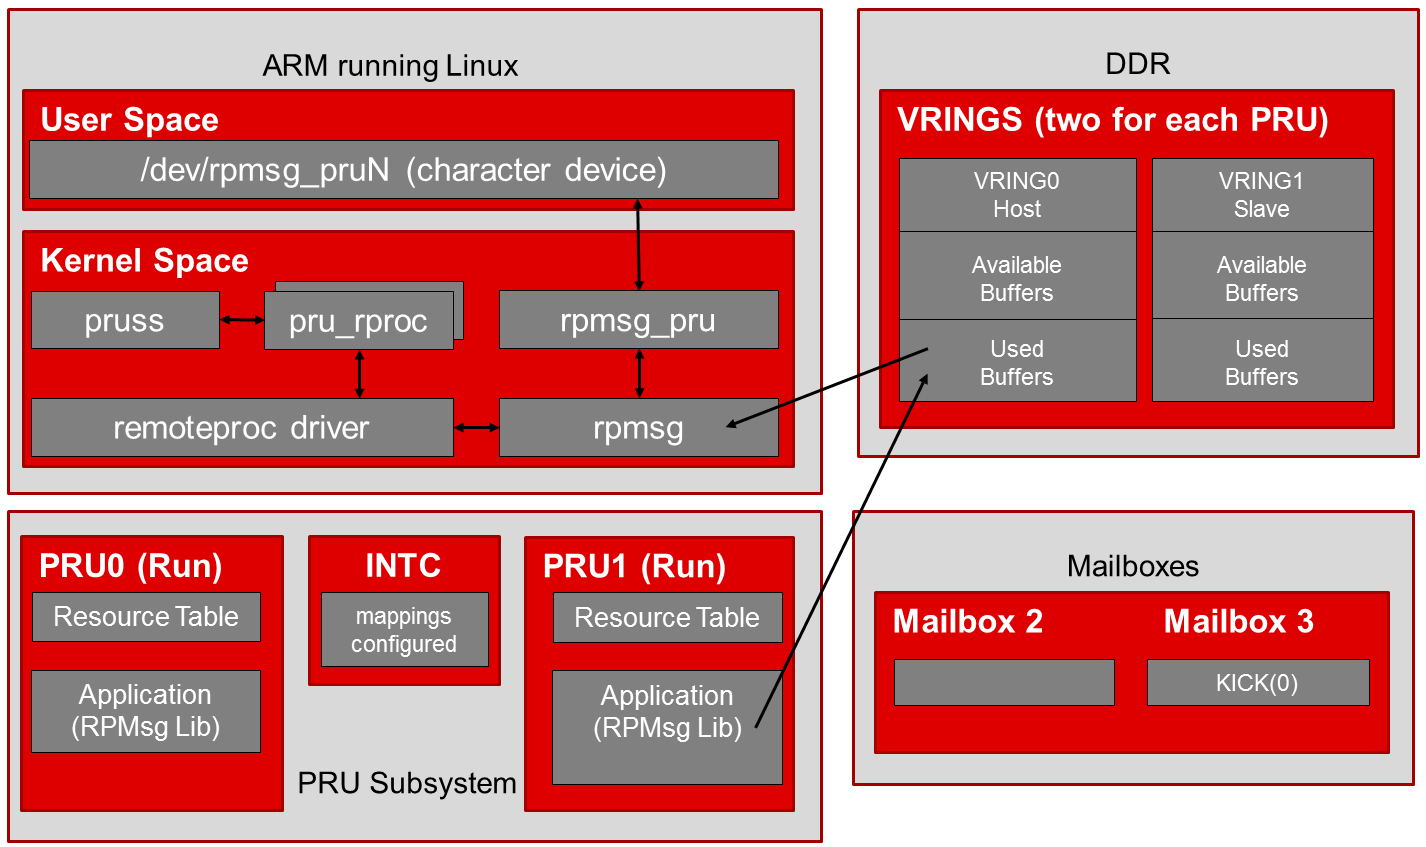
\includegraphics[width=0.8\textwidth]{IPC_linux_PRU_components.png}
    \caption{Components for Linux and PRU IPC}
\end{figure}

\subsubsection{ARM to PRU}

\begin{figure}[ht]
    \centering
    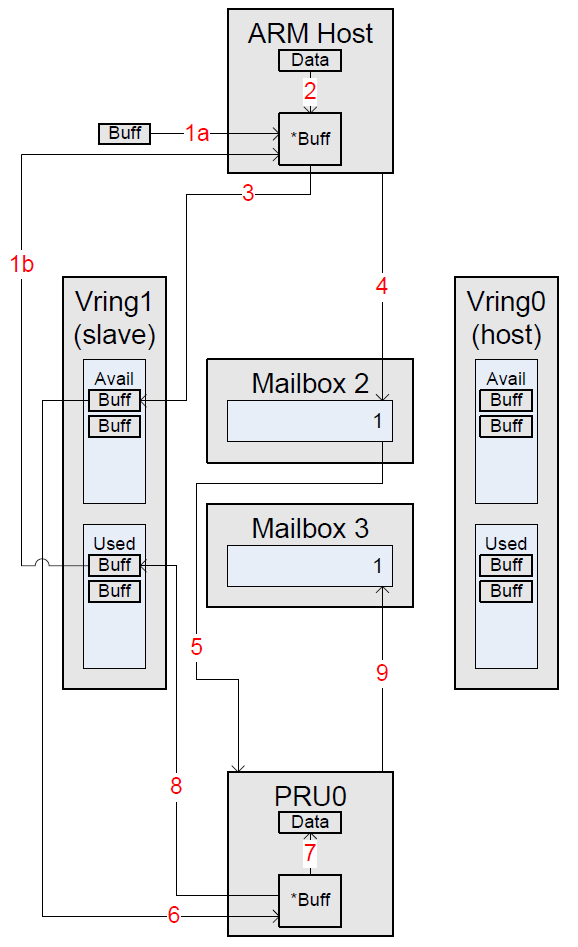
\includegraphics[width=0.6\textwidth]{IPC_linux_ARM_to_PRU.png}
    \caption{Steps needed to send a message from the ARM core to the PRU}
\end{figure}

Steps for the ARM core:

\begin{enumerate}
    \item   Allocate or Retrieve Buffer: the ARM host starts by either
            allocating or acquiring a used buffer from the slave Vring.
    \item   Data copy: the data to be transferred is copied into the chosen
            buffer.
    \item   Add to Available List: The filled buffer is then added to the
            available list in the slave Vring.
    \item   Notify the PRU: to signal the PRU, the ARM host kicks the slave
            Vring by sending its index via a message in Mailbox 2.
\end{enumerate}

Steps for the PRU core:

\begin{enumerate}
    \item   Detect Kick: The PRU monitors Mailbox 2 for a kick with the index
            of the relevant Vring, indicating that data is ready for reception.
    \item   Retrieve Available Buffer: the PRU obtains the available buffer
            from the slave Vring.
    \item   Data extraction: the data to be received is copied from the buffer
            in the previous step.
    \item   Add to Used List: the now empty buffer is added to the used list
            in the slave Vring.
    \item   Notify the ARM Host: to inform the ARM host about the completion,
            the PRU kicks the slave Vring by writing its index into a message
            in Mailbox 3.
\end{enumerate}

\subsubsection{PRU to ARM}

\begin{figure}[ht]
    \centering
    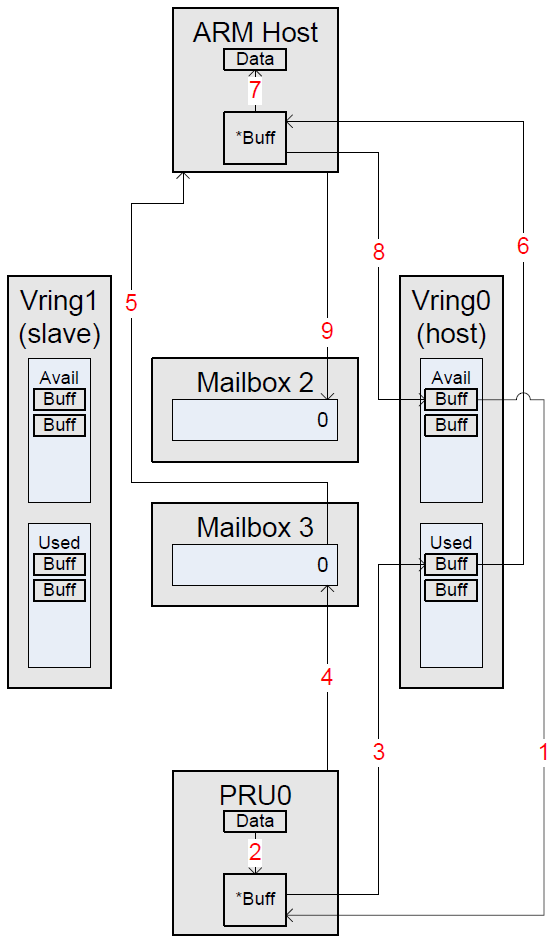
\includegraphics[width=0.6\textwidth]{IPC_linux_PRU_to_ARM.png}
    \caption{Steps needed to send a message from the PRU to the ARM core}
\end{figure}

Steps for the PRU:

\begin{enumerate}
    \item   Retrieve Available Buffer: the PRU starts by obtaining an
            available buffer from the host Vring.
    \item   Data copy: the data to be transferred is copied into the buffer 
            of the previous step.
    \item   Add to Used List: The filled buffer is then added to the
            used list in the host Vring.
    \item   Notify the ARM: to signal the ARM host, the PRU kicks the host 
            Vring by writing its index into a message in Mailbox 3.
\end{enumerate}

Steps for the ARM host:

\begin{enumerate}
    \item   Kicked Vring Detection: an interrupt is triggered, signaling that
            Mailbox 3 was kicked with the index of the host Vring.
            This notifies the ARM host that data is available for reception.
            of the relevant Vring, indicating that data is ready for reception.
    \item   Retrieve Used Buffer: the ARM host retrieves the used buffer
            from the host Vring.
    \item   Data extraction: the data to be received is copied from the buffer
            acquired in the previous step.
    \item   Add to Available List: the now empty buffer is added to the
            available list in the slave Vring.
    \item   Notify the PRU: to inform the PRU about the completion,
            the ARM host kicks the host Vring by writing its index into a
            message in Mailbox 2.
\end{enumerate}

\section{System boot}

The boot process is a complex process in the AM64x, since it has different
heterogeneous processors. An additional core, a Cortex-M3, is reserved for the
booting process and other management functions. This core is also called
Device Management and Security Controller (DMSC).

\subsection{Boot without Linux}

The bootflow, in case the A53 is not running Linux, consists of two main steps
that occur when the device is powered on:

\begin{enumerate}
    \item   ROM boot
    \item   SBL boot
\end{enumerate}

In the ROM boot step, a built-in component of microcontroller hardware, called
ROM bootloader, takes control. Its primary responsibility is to initiate the
next-stage bootloader, the SBL.
The ROM bootloader is generally kept in secure, read-olny memory to ensure its
integrity and security, working as root of trust for the rest of the operations.

After the ROM bootloader, the SBL takes control which is typically more
versatile and configurable than the ROM bootloader.
The SBL is responsible for orchestrating the boot process of the actual
application.
It can perform complex bootloading tasks, including initializing different
processor cores and managing the loading and execution of the application
software. It may also handle the parsing and loading of the application image
into the appropriate memory locations and take care of other initialization
tasks required for the application to run successfully.

\subsubsection{Initial Boot Flow}

The initial boot flow is the first part of the boot process and it specifies
how everything starts and how all the cores that belongs to the system are
initialized and started.

The core components to start the initial boot process are:

\begin{enumerate}
    \item   DMSC
    \item   R5F core
    \item   Boot pins
\end{enumerate}

The DMSC is a core dedicated for the central management of the device.
\cite{Technical_reference_AM64}
Upon powering the system, the DMSC is the first core that starts, executing 
the first set of instructions on the AM64X device, through the DMSC ROM code.
Subsequently, it will run the SYSFW code, which provides runtime functions that
help the system to be configured and run correctly.

The Cortex R5F acts as the boot controller of the system.
It is the core which manages the rest of the boot flow on the device, after it
has been released from reset by the DMSC. When it comes out of the reset, it
executes the R5 ROM code, and eventually it will run the SBL.

The boot pins are a set of pins in the board which specifies where the SBL
image is located and how the peripheral storing it is configured. 

\begin{figure}[ht]
    \centering
    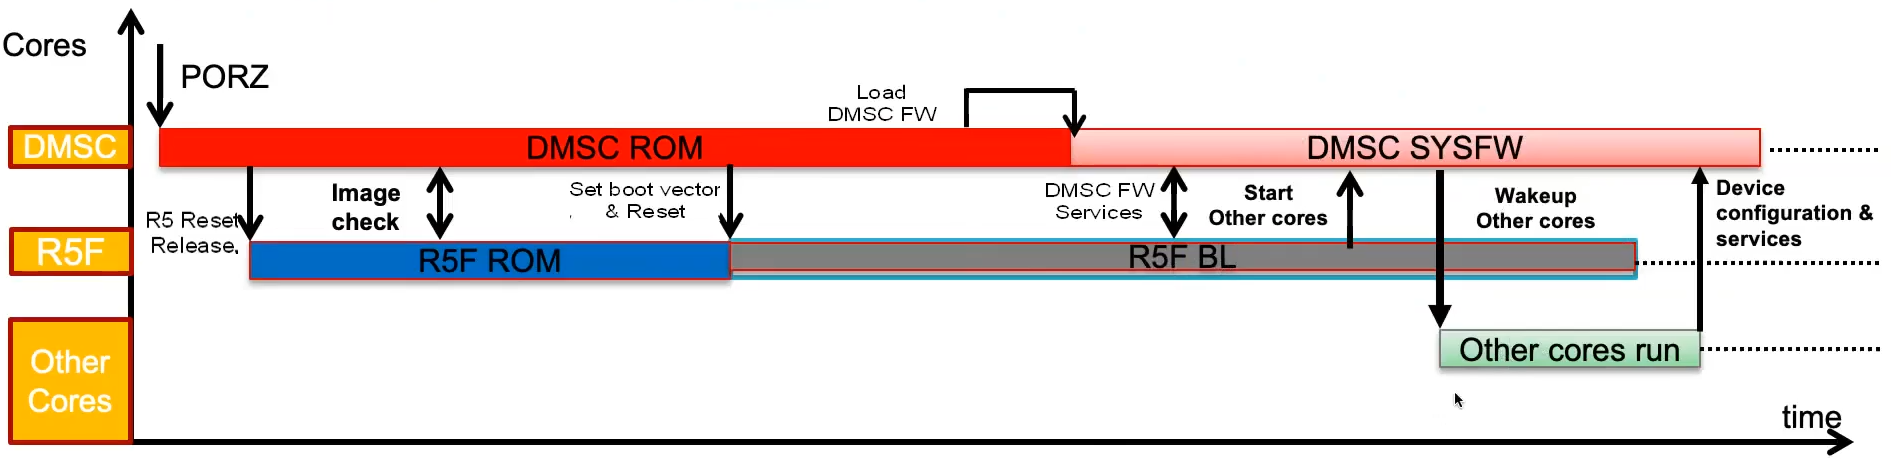
\includegraphics[width=1.0\textwidth]{boot_initial_flow.png}
    \caption{Initial boot flow of the SoC}
\end{figure}

The first thing after the Power On Reset (PORZ) is running the DMSC ROM, which
in turn starts the R5F ROM code. The two of them will collaborate to realize
the boot of the system.

After that, the SBL is needed for the boot process. The SBL will be loaded in
the R5 from the peripheral specified with the boot pins.
Before loading it, the DMSC validates the image's integrity. 
The R5 will find the image for the SYSFW, store it in its internal memory and
the DMSC will check that the firmware is valid before storing in its internal
memory and executing the code.

The next stages of the boot process will be done by the R5, in conjunction with
the services offered by the SYSFW. As the other cores start up, they will use
SYSFW services to check and configure the rest of the device.

\subsubsection{Boot Process flow}

\begin{figure}
    \centering
    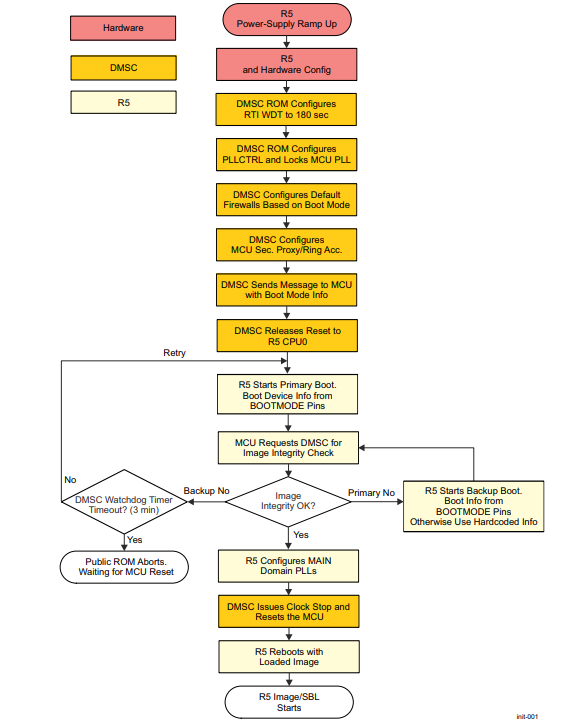
\includegraphics[width=0.8\textwidth]{boot_process_flow.png}
    \caption{Flow of the boot process}
\end{figure}

In the boot process, the DMSC works as the boot controller for the public ROM.
It takes care of essential configurations and releases the reset for R5's CPU.
The R5 core checks the boot mode pins and sets up the necessary peripheral
interface to access a boot image. After conducting a cursory image check, the
verified boot image is handed over to the DMSC.

The DMSC ROM then takes over, performing code verification and routing the boot
image to the on-chip RAM. Following this, the R5 core transitions into an idle
state. DMSC ROM code asserts a reset ot the MCU, redirects the boot vector to
the freshly loaded image, and releases the reset, thereby initiaing a restart
of R5. This restart occurs with the Public ROM code fully disconnected.

Finally, the execution of the Public ROM code is triggered after a cold or warm
reset, marking the completion of the boot process.

\begin{figure}
    \centering
    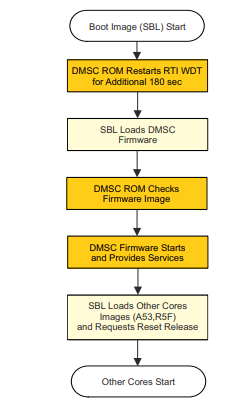
\includegraphics[width=0.4\textwidth]{boot_sbl_flow.png}
    \caption{Steps done by the SBL}
\end{figure}

Upon the reset of R5 and the initiation of SBL execution, the DMSC ROM performs
a restart of the RTI (Real-Time Interrupt) watchdog timer, extending the
timeout for an additional 180 seconds.
During this time, it becomes imperative for SBL to load the DMSC firmware
provided by Texas Instruments; failure to do so may result in a preemptive MCU
reset, serving as a protective measure against potential software misbehavior.

One of the primary responsibilities of SBL is to load the DMSC firmware.
Only after successfully executing this task can SBL proceed to load the images
for other processors and request a reset release from the DMSC firmware for
those cores.

\subsection{DMSC}

The DMSC performs the following functions:

\begin{itemize}
    \item   Device Management
    \item   Configuration of boot vectors and control of the reset release
            of the R5 core
    \item   IPC configuration via main DMSS rings and Secure Proxy
    \item   PLL configuration (R5 and SA2UL)
    \item   X509 certificate parsing
    \item   SA2UL configuration to SHA512 for image integrity checks
    \item   DMSC fimware loading
\end{itemize}

In the case of AM64X the firmware loaded by the DMSC is the System Controller
Firmware (SYSFW). It acts as a centralized server for the SoC. The services it
provides are:

\begin{itemize}
    \item   Resource Management: SYSFW manages system resources, ensuring that
            various hardware components and resources are allocated, accessed,
            and controlled efficiently. This includes tasks such as configuring
            and managing peripherals, memory regions, and interconnects. It is
            essential to avid conflicts between different components of the SoC.
    \item   Power Management: SYSFW is responsible for controlling the power
            states of different parts of the SoC. It manages power modes and
            transitions, ensuring that the SoC operates in power-efficient
            states when possible.
    \item   Security: SYSFW enforces security policies, handling secure boot
            processes, and managing cryptographic functions to protect the
            system from unuathorized access or tampering. It may be involved in
            setting up and managing hardware security features.
\end{itemize}

Given the importance of the task performed by the SYSFW, it needs to be loaded
and executed before the Secondary Bootloader (SBL) or any other part of the
system can perform their tasks effectively.

\subsection{Linux boot}

The initial boot flow is similar to the one presented before, even if Linux
has to be run.
The DMSC always runs the SYSFW and starts the booting process.
The R5F will start loading all the images for the necessary components of the
system: ATF, OPTEE, and A53 SPL, all coming from the boot media, specified
through the boot pins.

\begin{enumerate}
    \item   ATF: ARM Trusted Firmware, is a software component that secures
            booting, manages hardware, and establishes trusted environments
            on Arm-based systems.
    \item   OPTEE: establishes a secure environment on Arm-based systems for
            running and managing trusted applications, ensuring isolation and
            security from the normal system operations.
    \item   A53 SPL: small piece of code or bootloader necessary for
            initializing the system hardware, which will run on the A53 core.
\end{enumerate}

\begin{figure}[ht]
    \centering
    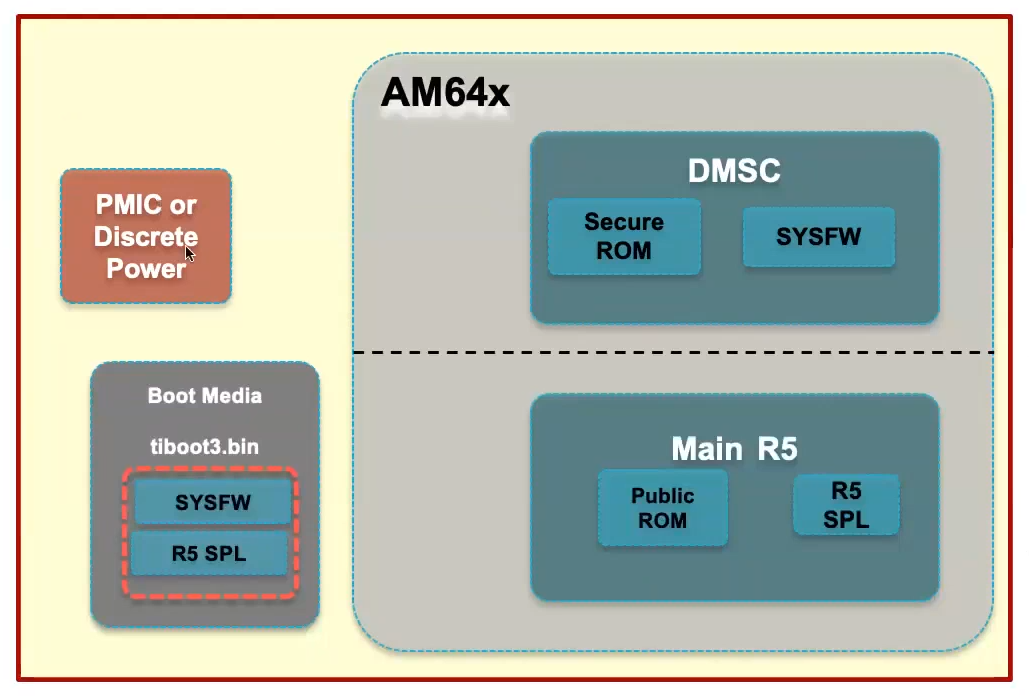
\includegraphics[width=1.0\textwidth]{boot_linux_components.png}
    \caption{Components needed for the boot of Linux}
\end{figure}

\begin{figure}[ht]
    \centering
    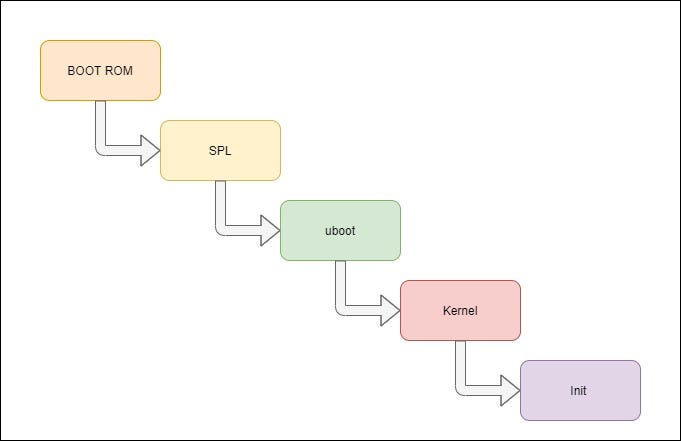
\includegraphics[width=0.8\textwidth]{boot_linux_flow.jpg}
    \caption{Linux Boot Flow}
\end{figure}

The ROM copies content of the bootloader to static RAM. SRAM memory is limited,
due to physical reasons and we only have few KBs for bootloader.
Usually, regular bootloader (e.g. U-Boot) binary is bigger than that.
So we need to create some additional bootloader, which will initialize regular
RAM and copy bootloader to RAM, and then jump to execute that regular
bootloader. This additional bootloader is usually referred as uboot-SPL
(which stands for Secondary Program Loader).

The bootloader (uboot) decompresses the Linux kernel into RAM from the
specified peripheral. It then executes a jump to the kernel's first
instruction, starting the execution of the system.


